\documentclass{article}

\usepackage{booktabs}
\usepackage{multirow}
\usepackage{graphicx}
\usepackage{geometry}
\geometry{margin=1in}
\usepackage{float}

\title{HW\#2}
\author{Jeremy First}
\date{2015-10-20}

\begin{document}

\begin{center}

\Large\textbf{Homework \#2}\\
\large\textbf{Jeremy First}\\
\large{06 November 2015}
\end{center}

\section{Exercise 2.0 - Compiling a 3rd Party Library}
The GSL library was compiled in 4 different configurations, both in serial and parallel. The compilation times are listed in Table \ref{tab:times}. 

\begin{table}[h!]
	\begin{center}
	\label{tab:times}
	\begin{tabular}{|c||c|c|c|c|}
		\hline
		\multirow{2}{*}{Configuration} & \multicolumn{2}{ c }{Compilation Tests} & \multicolumn{2}{|c|}{Regression Tests} \\
		& Serial(secs) & Parallel(secs) & Passes & Failures \\
		\hline
		\cline{1-5}
		gcc/noOpt & 88.271 &  21.310 & 48 & 0\\
		gcc/O3 & 180.975 &  41.633 & 48  & 0\\
		icc/noOpt & 300.187 & 47.419 & 48 & 0 \\
		icc/O3 & 315.618 & 77.081 & 44 & 4 \\
		\hline
	\end{tabular}
	\caption{\small{Compilation time and regression tests for four different configurations of the GSL library.} }
	\end{center}
\end{table}

As you can see in Table \ref{tab:times}, the Intel compiler is significantly slower than the GNU compiler.  In serial, with no optimization, the GNU compiler is more than three times as fast. In parallel however, this difference decreases to twice as fast, suggesting that the Intel compiler runs more efficiently in parallel than the GNU compiler. With -O3 optimization, the GNU compiler still outperformed the Intel compiler at a little less than twice as fast. In parallel with -O3, the GNU compiler remained about twice as fast as the Intel compiler. 

The GNU compilation time with no optimizations decreased four-fold from serial to parallel compilation. 
 
 \section{Exercise 2.1 - Simple Makefile}
 
A Makefile is included in the submitted tar ball.  Note that the GSL module must be loaded before running make. 
\begin{verbatim}
module load gsl 
make 
\end{verbatim}
 
 \section{Exercise 2.2 - Revisiting numerical integration}
 
 Note that the boost module must be loaded before running my program. 
 \begin{verbatim}
 module load boost
 make CC=icc
 ./Exc2.2 -a 0 -b 5 -n 100
 \end{verbatim}
 A C++ program was written to evaluate the numeric integral of $f(x)=cos(x)$. The program accepts three command-line arguments that control the limits and discretization level, and a fourth option ``-h'' to display information about the program. The code also prints the absolute error between the numerical solution and the exact analytic solution. The program is contained in the subdirectory Exc2.2 of the submitted tar ball, and has an included Makefile. The program is dependent on the Boost libraries, so the Boost module must be loaded to build and run the program on Stampede. 
 
 The following cases were run for the limits $[x_{min}, x_{max}] = [0.0,5.0]$ and the run-time performance was timed:
 \begin{itemize} \itemsep1pt \parskip0pt \parsep0pt
 \item NP=10
\item NP=50
\item NP=100
\item NP=200
 \end{itemize}
 These run-time performances are shown in Figure \ref{fig:run-times}, compared to the run-time performances of the same program, written in bash. 

  \begin{figure}[H]
  \begin{center}
  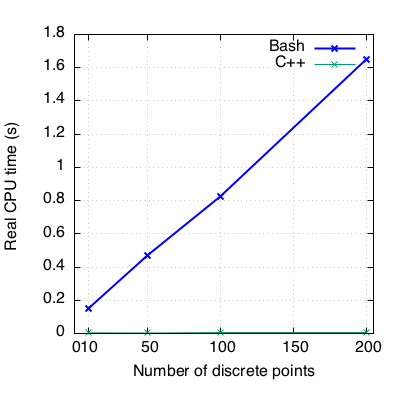
\includegraphics[scale=0.4]{Exc2.2/times_vs_numPoints.png}
  \caption{\small{Run-time performance of a numerical integration of $\int_0^5\cos(x)$, written in both bash (blue) and C++(green). Note that in C++, the run-time performance stayed very close 0.005 s for each of the four trials, and the line lays flat along the x-axis.}}
  \label{fig:run-times}
  \end{center}
  \end{figure}
  
  As can be seen from Figure \ref{fig:run-times}, no appreciable increase in time can be seen in the C++ for these levels of discretization. Since this figure is very boring to look at, the run-time performance was timed again for much larger levels of discretization. An appreciable increase in run-time could not be measure until 10000 steps were used. At this level of discretization, the absolute error is $< 10^{-6}$. Figure \ref{figure:largen} shows run-time performance for large values of n. 
  
  \begin{figure}[H]
  \begin{center}
  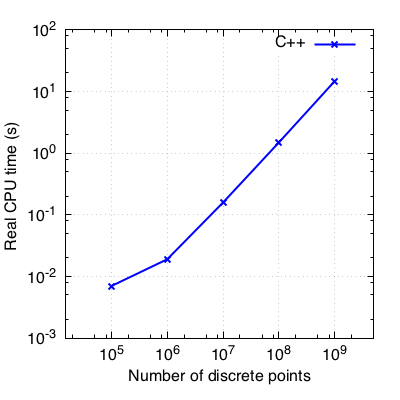
\includegraphics[scale=0.4]{Exc2.2/times_vs_largen.png}
  \caption{\small{Run-time performance at very large discretization levels. At these levels, the absolute error has dropped below $10^{-6}$ . }}
  \label{figure:largen}
  \end{center}
  \end{figure}
  
  The absolute errors are plotted in Figure \ref{fig:errors}. 
  \begin{figure}[H]
  \begin{center}
  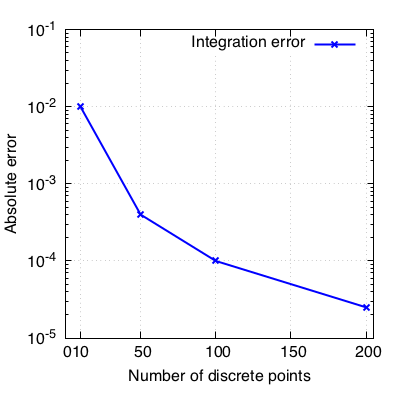
\includegraphics[scale=0.4]{Exc2.2/error_vs_numPoints.png}
  \caption{\small{Absolute error of a C++ numerical integration of $ \int_0^5 \cos(x) dx. $}}
  \label{fig:errors}
  \end{center}
  \end{figure}
  
  We see the same rate of convergence as we did last week with the bash script. 
  
  \section{Exercise 2.3 - Sterling's approximation}
  A C++ program was written to calculate the error in Sterling's approximation for every integer between 1 and 100. The program is included in the Exc2.3 subdirectory of the submitted tar ball. It includes a Makefile to build the program. The programs, prints $N$, $ln(N!)$, and the absolute error of Sterling's approximation, $\ln(N!)=N \cdot \ln(N) - N$. The errors is plotted in Figure \ref{fig:sterling}. 
  \begin{figure}[H]
  \begin{center}
  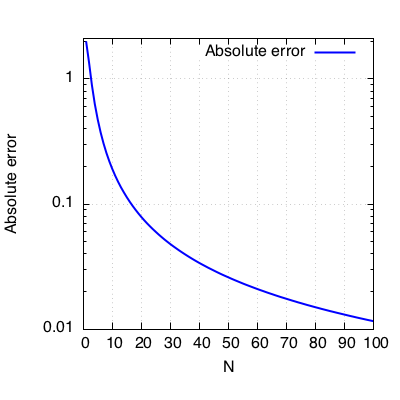
\includegraphics[scale=0.4]{Exc2.3/stirling_error.png}
  \caption{\small{The absolute error of Stirling's approximation against the number of terms.} }
 \label{fig:sterling}
  \end{center}
  \end{figure}
To figure out the number of terms that would have an error of less than 0.1\%, the program was modified to loop through integers until the error was less than 0.1\%. At $N=915$, the error is 0.100\%. Therefore, for $N>915$, the error is less than 0.1\%. 

\section{Exercise 2.4 - More one-liners}
\begin{itemize}
\item Count how many files have been modified in your home directory in the last 24 hours. 
\begin{verbatim}
find . -Btime 0 | wc -l 
\end{verbatim}

\item Suppose you have no morals and want to ruin somebody's day. Provide a one liner that will replace all tab characters in a Makefile by spaces.
\begin{verbatim}
cat Makefile | expand > new_Makefile ; mv new_Makefile Makefile
\end{verbatim}
\item Print the 50th line of a file named sample.txt 
\begin{verbatim}
head -n 50 sample.txt | tail -n 1
\end{verbatim}
\item Create a simple stopwatch from an infinite while loop. 
\begin{verbatim}
i=1 ; while(true) ; do sleep 1 ; echo $i ; ((i++)) ; done 
\end{verbatim}
\item How many hidden files are in your home directory and it's subdirectories?
\begin{verbatim}
find . -name ".*" | wc -l 
\end{verbatim}
\end{itemize}
	

 \end{document}

